%!TEX root = ../luanvan.tex
\chapter{Xây dựng hệ thống}
\section{Tổng quan giải pháp}

Problem Statement
Every school/university around has its way of managing or maintaining its student records and transcripts. Of course, many of them usually do not share student information, such as transcripts for privacy reasons. Typically, in the case of international students, when one student tries for an admission in a foreign country, the student must get his transcripts evaluated by a third-party evaluator such as WES, an International evaluator.

For one reason, if somehow these transcripts are in a foreign language, there needs a
translator and, most of the time requires to approach a third-party evaluator. When a person had started applying for a university in the United States, The university required him to first apply all the transcripts from his school and then had them evaluate through an external evaluator to match the grading system between the two countries, and it takes an average of 2-3 weeks to get the evaluation report. Table 1 is the third-party evaluator's cost summary.
So, a cryptographic database solution for recording the academic certificates will help to solve all these issues. By making all the official and unofficial transcripts of the student store in a blockchain, which are accessible through all over the world and can share to any Employer or a University And the transcripts stored on a blockchain system are immutable, therefore preserves the integrity of data.

Objective of the Study
To develop an application on a blockchain framework, which is a role-based access system, takes inputs and stores all the changes performed on it, which supports an authentication system and high scalability.

Hệ thống quản lý VBCC sử dụng công nghệ blockchain có các chức năng: cấp, quản lý và xác minh VBCC một cách an toàn, bảo mật. Giải pháp được thử nghiệm với nền tảng kỹ thuật số của IBM Blockchain Flatform, Hyperledger Fabric. VBCC có thể được xác thực với tùy chọn hạn chế tiết lộ thông tin và không cần sự can thiệp từ tổ chức cấp chứng chỉ (Trường/Trung tâm).

\begin{figure}[htbp]
\centering
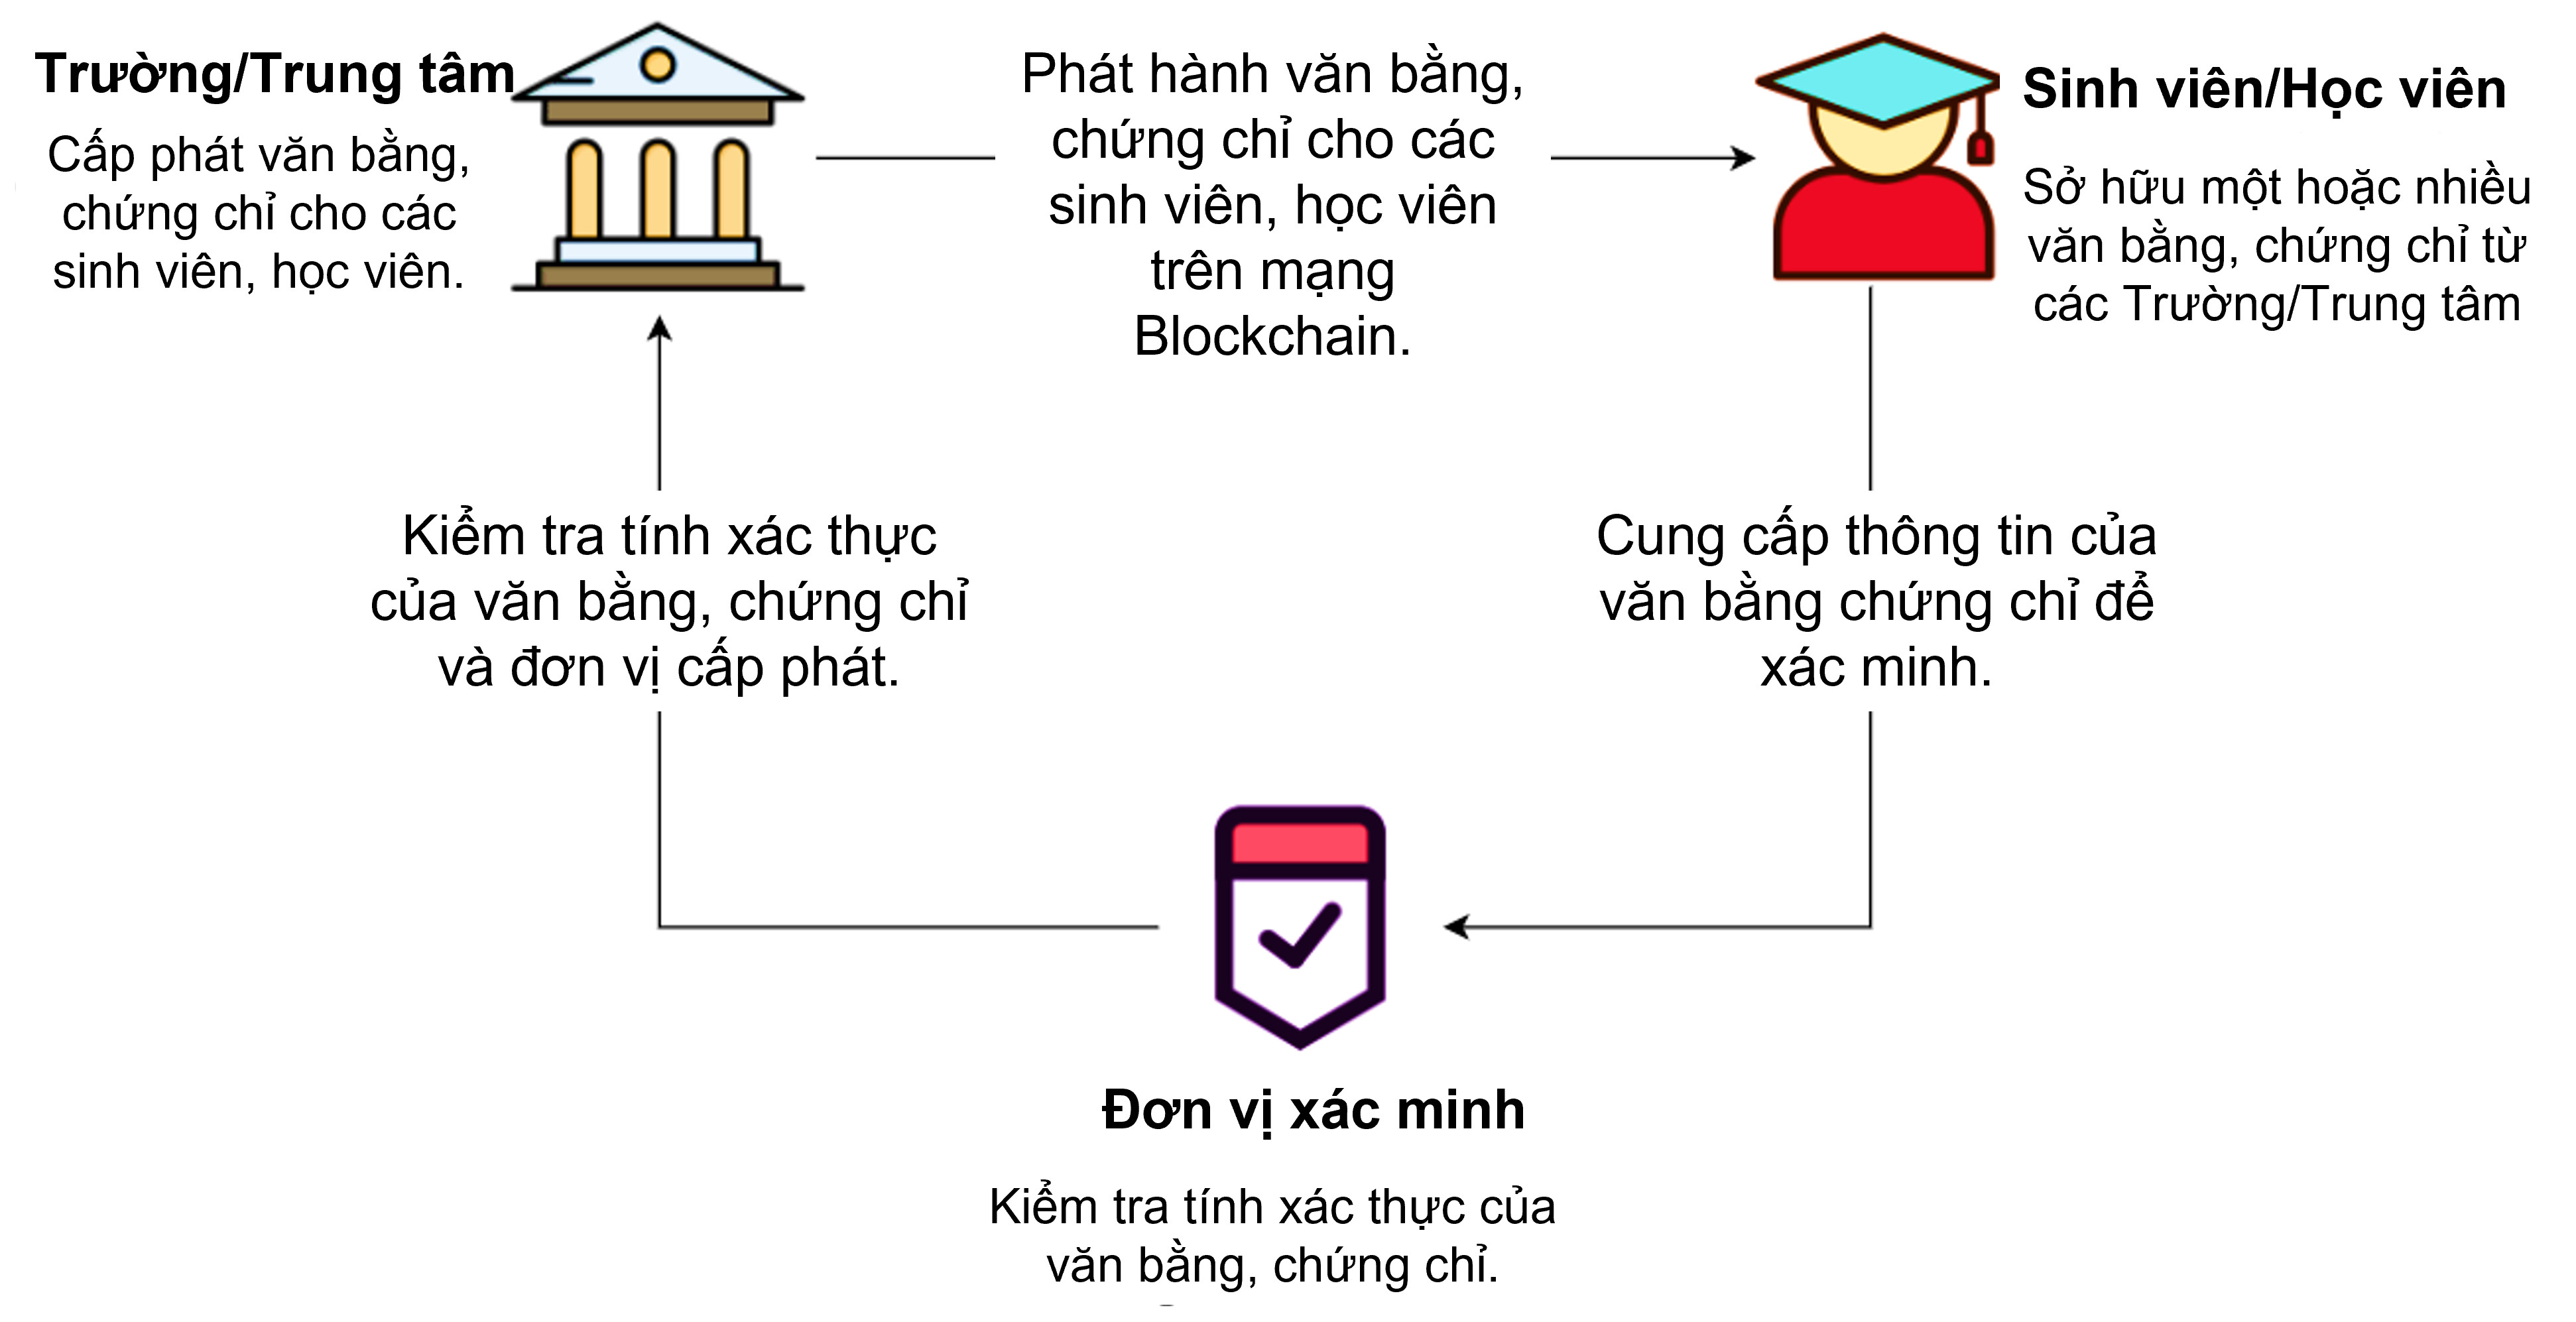
\includegraphics[width=.9\linewidth]{img/vbcc.jpg}
\caption{Sơ đồ tổng quan giải pháp}
\label{fig:vbcc}

\end{figure}
Những chức năng chính của hệ thống được mô tả như hình \ref{fig:vbcc} bao gồm:
\begin{itemize}
\item Trường/Trung tâm: ký số và cấp VBCC.
\item Sinh viên: xem và chia sẻ VBCC.
\item Đơn vị xác minh: kiểm tra tính xác thực của các VBCC được chia sẻ.
\end{itemize}


\section{Kiến trúc phần mềm}
Kiến trúc phần mềm được mô tả như hình \ref{fig:vbcc_phanmem} bao gồm các thành phần:
\begin{figure}[htbp]
\centering
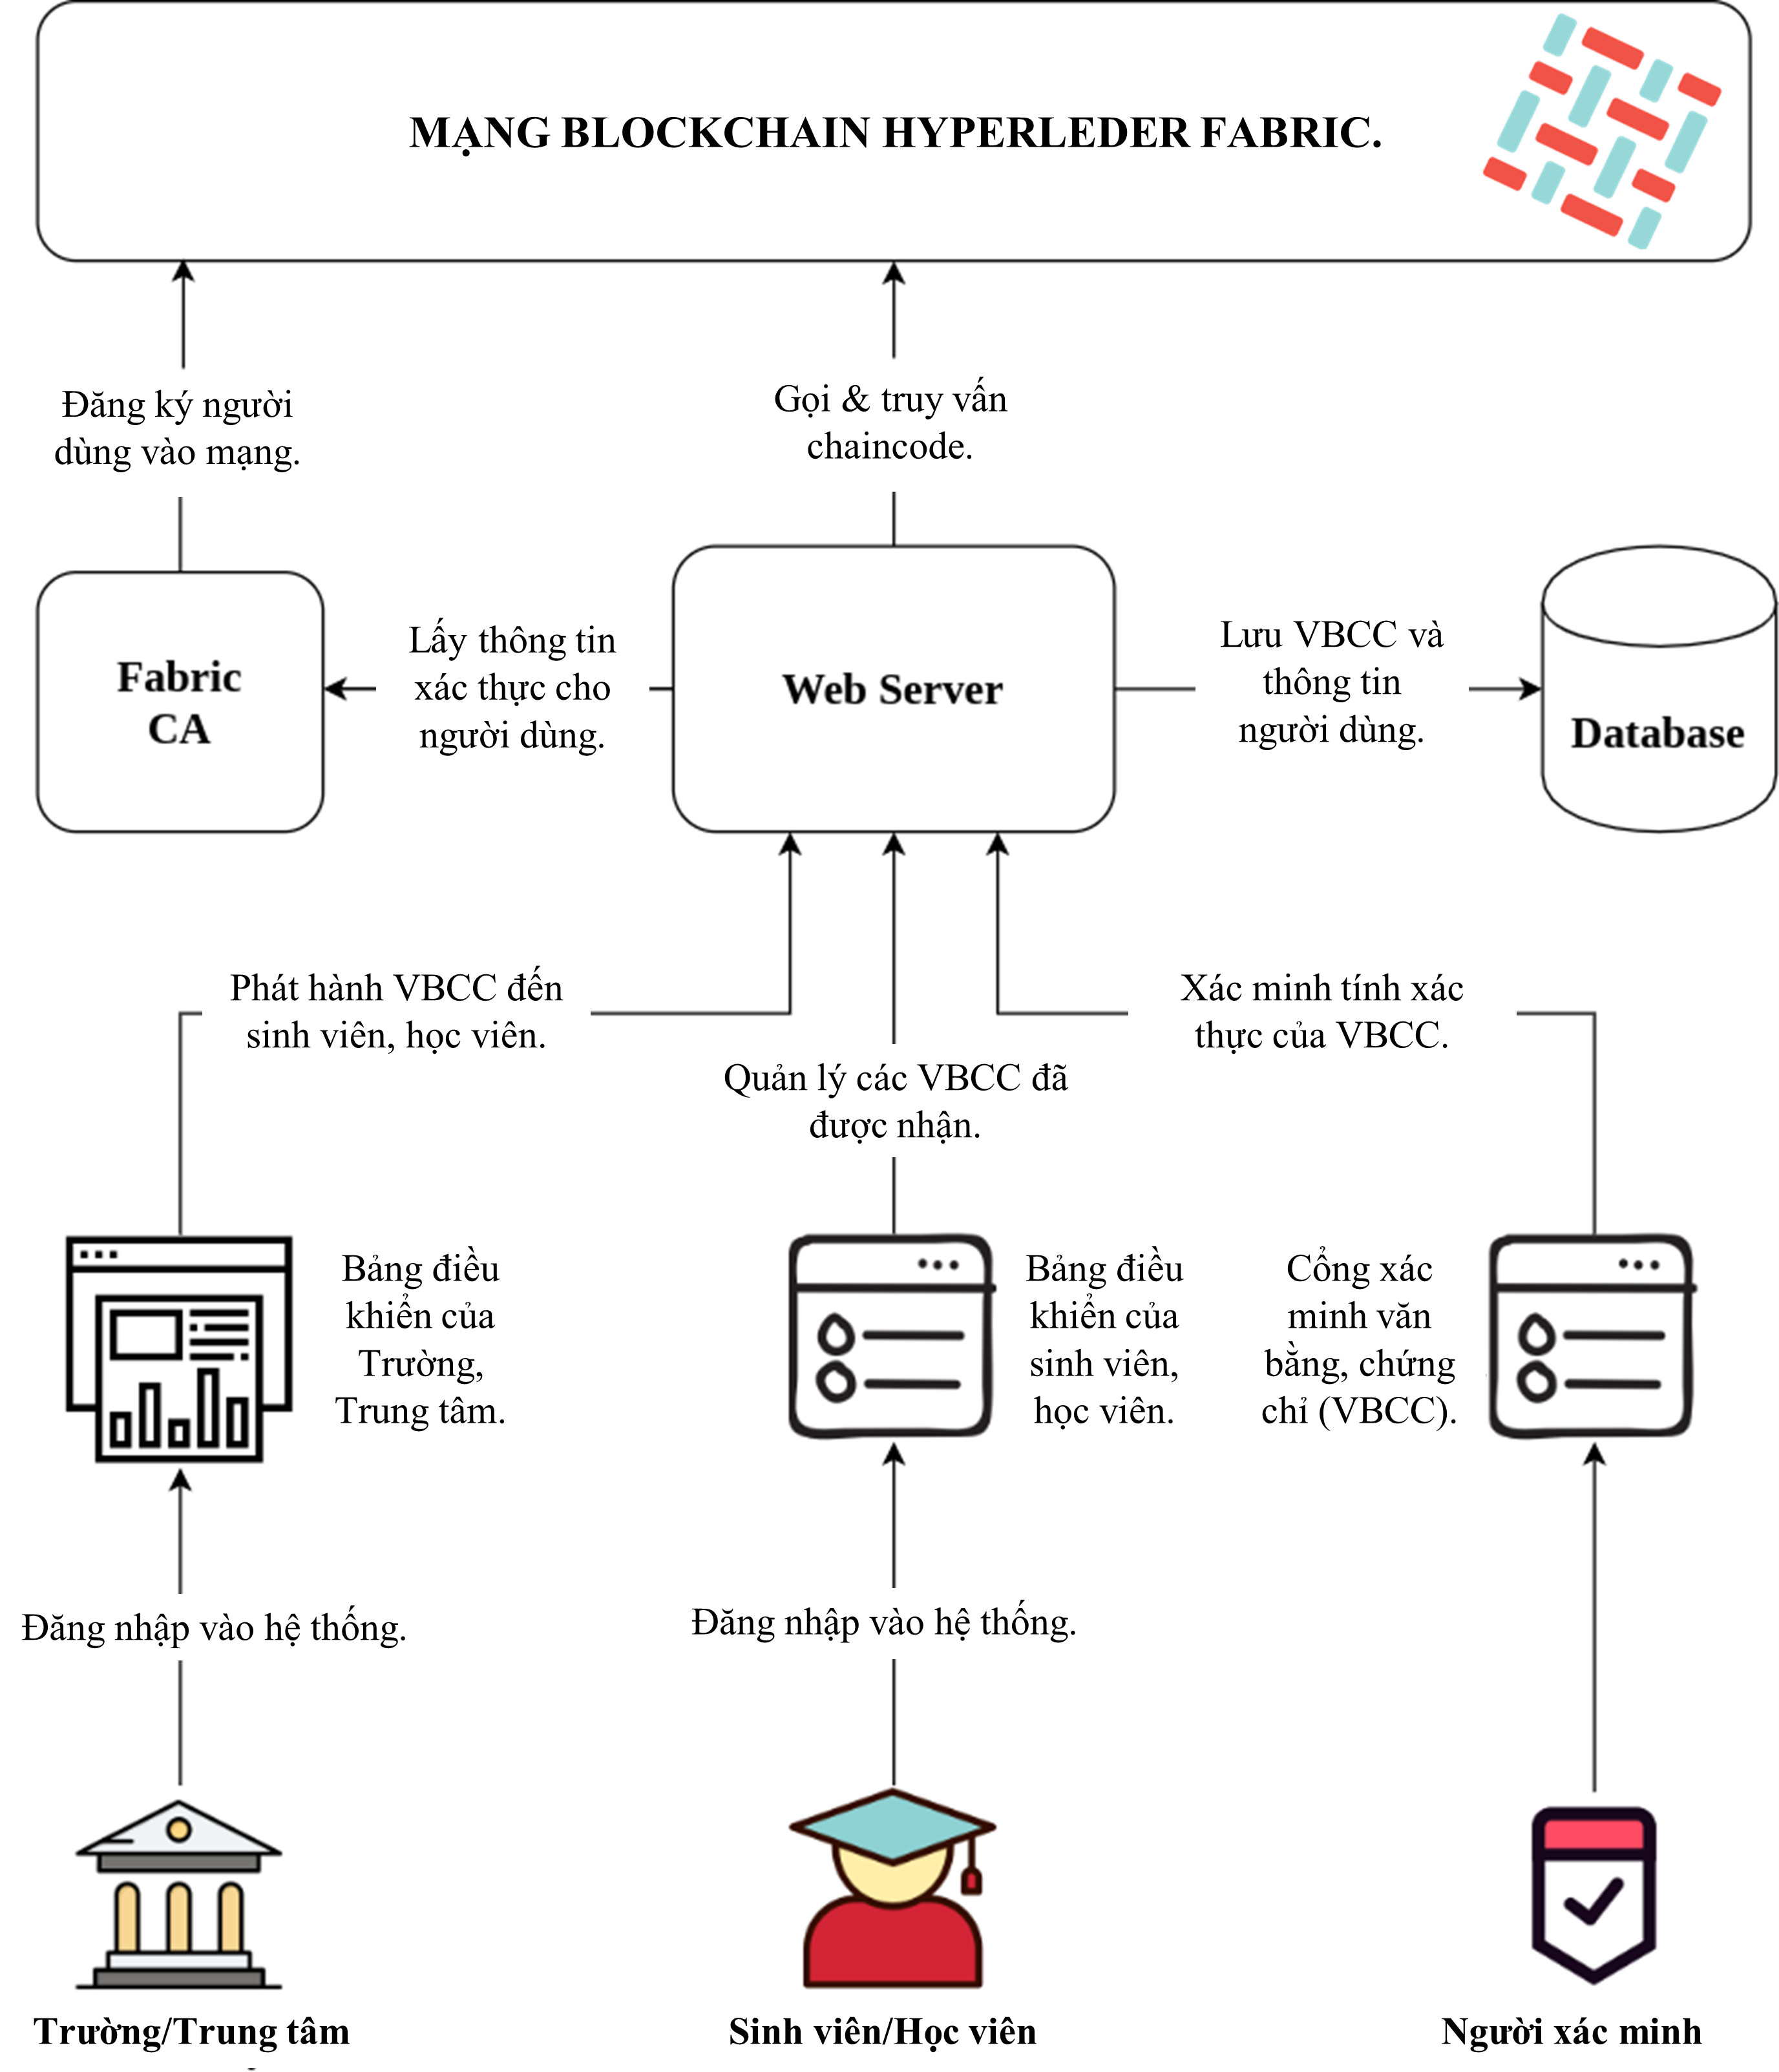
\includegraphics[width=.9\linewidth]{img/vbcc_phanmem.jpg}
\caption{Sơ đồ kiến trúc phần mềm}
\label{fig:vbcc_phanmem}
\end{figure}
\begin{enumerate}
\item Mạng Blockchain Hyperledger Fabric: IBM Blockchain Flatform và Docker container hỗ trợ xây dựng mạng blockchain Fabric, thực thi các hợp đồng thông minh (ngôn ngữ Javascript).
\item Fabric CA: được dùng để đăng ký và xác thực các thành phần trong mạng.
\item Webserver: sử dụng Node.js cung cấp giao diện Backend của ứng dụng web, kết hợp sử dụng Nodejs Express.
\item Cơ sở dữ liệu MongoDB: lưu trữ dữ liệu người dùng và chứng chỉ.
\item Giao diện Front-end của ứng dụng web: dùng các thư viện Bootstrap, jQuery.
\end{enumerate}

\section{Các thành phần tham gia}
Các thành phần tham gia của hệ thống bao gồm: (1) Trường, Trung tâm, (2) Sinh viên (học viên) và (3) Bên xác minh chứng chỉ (Ví dụ: nhà tuyển dụng). Mỗi thành phần sẽ có các hành động như sau:

\emph{Trường, trung tâm}

\begin{itemize}
\item Đăng ký tài khoản.
\item Đăng nhập tài khoản.
\item Cấp VBCC có xác nhận chứng thực và ký số VBCC.
\item Xem VBCC đã cấp.
\end{itemize}

\emph{Sinh viên, học viên}

\begin{itemize}
\item Đăng ký tài khoản.
\item Đăng nhập tài khoản.
\item Xem VBCC đã nhận.
\item Chia sẻ thông tin VBCC.
\item Tiết lộ thông tin VBCC có chọn lọc nhằm hạn chế lộ thông tin.
\end{itemize}

\emph{Bên xác minh chứng chỉ}

\begin{itemize}
\item Xác minh tính xác thực của VBCC với nền tảng blockchain.
\end{itemize}


Quy trình hoạt động của hệ thống được mô tả như hình \ref{fig:vbcc_diagram}

Mô tả quy trình hoạt động
\begin{figure}[htbp]
\centering
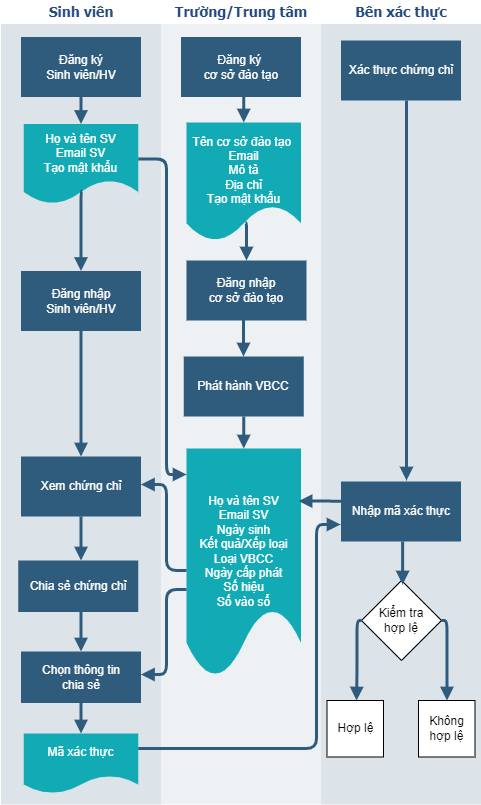
\includegraphics[width=.9\linewidth]{img/vbcc_diagram2.png}
\caption{Quy trình hoạt động của hệ thống}
\label{fig:vbcc_diagram}
\end{figure}
\subsection{Mô tả usecase}
\subsection{Thiết kế cơ sở dữ liệu}
\subsection{Thiết kế mạng blockchain}

Mô tả các asset

Mô tả smartcontract

Mô tả cài mạng Hyperledger Fabric

